\documentclass[12pt,a4paper]{report}

% --- Языковая и шрифтовая настройка ---
\usepackage[T2A]{fontenc}
\usepackage[utf8]{inputenc}
\usepackage[english,russian]{babel}
\usepackage[russian]{cleveref}

% --- Математика ---
\usepackage{amsmath,amssymb,amsthm}

% --- Рисунки и таблицы ---
\usepackage{graphicx}
\graphicspath{{img/}}
\usepackage{booktabs,array,caption}

% --- Сноски, гиперссылки ---
\usepackage[hidelinks]{hyperref}

% --- Библиография через biblatex ---
\usepackage[
  backend=bibtex,
  style=gost-numeric
]{biblatex}
\addbibresource{bibliography.bib}

% --- Параметры страницы ---
\usepackage[
  left=3cm,
  right=1.5cm,
  top=2cm,
  bottom=2cm
]{geometry}

% --- Информация для титульного листа ---
\newcommand{\University}{НИУ ВШЭ СПБ}
\newcommand{\Faculty}{ПАДИИ, 2 курс}
\newcommand{\Author}{Иванов~И.\,И.}
\newcommand{\Supervisor}{Петров~П.\,П., д.\,ф.-м.\,н., доцент}
\newcommand{\Title}{Отчёт об исследовательской работе:\\«Применение случайных графов для проверки гипотезы согласия»}
\newcommand{\Year}{2025}

\begin{document}

% === Титульный лист ===
\begin{titlepage}
  \centering
  {\large \University\par}
  \vspace{1cm}
  {\large \Faculty\par}
  \vfill
  {\Large \textbf{\Title}\par}
  \vfill
  {\large Студенты: Пожидаев Филипп, Афоничев Артемий}
  \vfill
  {\large \Year\par}
\end{titlepage}

% === Оглавление ===
\tableofcontents
\clearpage

% === Глава 1: Введение ===
\chapter{Введение}
Отчёт работы по исследованию свойств случайных графов (\texttt{KNN} и дистанционных), построенных на основе различных вероятностных распределений.\\
Цель работы: исследовать поведение числовых характеристик случайных графов в зависимости от параметров распределений и параметров построения графов.\\
Задачи:
\begin{enumerate}
  \item Изучить поведение числа треугольников, хроматического и кликового числа в зависимости от параметров распределений;
  \item Исследовать влияние параметров процедуры построения графа и размера выборки;
  \item Провести эксперименты с ML классификаторами.
\end{enumerate}

% === Глава 2: Описание кода ===
\chapter{Описание кода}
В данной главе мы рассмотрим алгоритмы и реализованные функции для проведения экспериментов.
\section{Построение \texttt{KNN}-графа и дистанционного графа, работа с их характеристиками}
\subsection{\texttt{KNN}-граф}
Функция \texttt{build\_knn\_graph(k, vertices)} реализует алгоритм построения \texttt{KNN}-графа на основе заданного набора вершин \texttt{vertices} и параметра $k$, определяющего количество ближайших соседей для каждой вершины.\\
Используется алгоритм \texttt{NearestNeighbors} из библиотеки \texttt{scikit-learn}, который для каждой вершины находит $k + 1$ ближайших соседей (включая саму вершину).
Создаётся граф с помощью библиотеки \texttt{networkx} \texttt{(nx.Graph())}.
\subsection{Дистанционный граф}
Функция \texttt{build\_distance\_graph(d, vertices)} строит граф, в котором вершины соединяются рёбрами, если расстояние между ними не превышает заданного порога $d$.
Для каждой пары вершин $(i, j)$ проверяется условие $|\texttt{v[$i$]} - \texttt{v[$j$]}| \le d$. Если условие выполняется, между вершинами добавляется ребро.
\subsection{Характеристики}
Функция \texttt{compute\_stats(arr)} вычисляет основные статистики массива данных: среднее значение, дисперсию, стандартное отклонение и стандартную ошибку.\\
Функции, предназначенные для вычисления минимальной степени, количества треугольников, хроматического числа, кликового числа, размера максимального независимого множества, числа доминирования, минимального размера кликового покрытия являются обёрткой над существующими в \texttt{networkx} методами класса \texttt{nx.Graph}.
\section{Распараллеливание метода Монте-Карло}
В данном разделе описывается реализация метода Монте-Карло с использованием параллельных вычислений для эффективного статистического анализа графовых структур. Предложенный подход позволяет ускорить проведение множественных экспериментов за счёт распределения вычислений между несколькими ядрами процессора.\\
Алгоритм состоит из двух основных функций. Они принимают следующий набор аргументов — \texttt{n, distr\_param, graph\_param, gen\_func, graph\_func, res\_func} (однако, второй в самом начале на вход ещё подаётся параметр \texttt{M}).
\subsection{\texttt{monte\_carlo\_step()}}
Выполняет отдельное испытание (одно повторение метода Монте-Карло). Является атомарной операцией для параллелизации.\\
Выполняет следующие шаги для одного испытания:
\begin{enumerate}
    \item Генерирует набор вершин с помощью функции \texttt{gen\_func} с заданными параметрами распределения \texttt{distr\_param};
    \item Строит граф указанным методом (\texttt{graph\_func}) с параметром \texttt{graph\_param};
    \item Вычисляет и возвращает требуемую характеристику графа с помощью функции \texttt{res\_func}.
\end{enumerate}
\subsection{\texttt{monte\_carlo\_multiprocessing()}}
Организует параллельное выполнение множества испытаний. Использует библиотеку \texttt{joblib} для распараллеливания, задействует все доступные ядра процессора, а результат всех испытаний собирает в единый массив.
\section{Параллельная генерация датасета}
В данном разделе описывается алгоритм параллельной генерации датасета для исследования характеристик случайных графов. Реализация использует многопоточные вычисления для эффективного создания большого объема данных.
\subsection{\texttt{generate\_row(idx, seed)}}
Генерирует дистанционный граф на $n$ вершинах ($n$ выбирается случайно из заданного набора $N$), считает ключевые характеристики.
\subsection{\texttt{generate\_dataset(num\_samples, seed)}}
Использует все ядра процессора, автоматически распределяет задачи, выводит прогресс бар с помощью модуля \texttt{tqdm}, собирает результат в единый \texttt{pd.DataFrame}.

% === Глава 3: Описание экспериментов ===
\chapter{Описание экспериментов}
Теперь перейдем к самим экспериментам.
\section{Исследование, как ведет себя числовая характеристика графа в зависимости от параметров процедуры построения графа}
В случае с дистанционным графом было установлено, что при росте $n$ и $d$ числовая характеристика и метрики качества растут, но у $d$ есть критический порог, после которого метрики растут незначительно или же вовсе не растут, этот порог для большинства $n$ равен $d = 0.8$. Это касается всех распределений (\texttt{Exp, LogNormal, Normal, SkewNormal}), но при анализе \texttt{Normal} и \texttt{SkewNormal} был замечен сдвиг порога ближе к единице.\\
Дальнейшее исследование проводилось с фиксированным $d$, равным:
\begin{itemize}
    \item 0.8 для \texttt{Exp, LogNormal};
    \item 0.9 для \texttt{Normal, SkewNormal}.
\end{itemize}
В \texttt{KNN}-графе было замечено, что метрики качества сильно зависят от $n$, а при больших $n$ качество оказалось не хуже, чем в дистанционном графе, поэтому именно он будет участвовать в дальнейших экспериментах, начиная с исследования важности характеристик для классификации.\\
Стоит отметить, что изначальные попытки извлечения какой-то информации о \texttt{KNN}-графе из его минимальной степени вершины являются артефактом условия исследовательской работы, поэтому было принято решение рассмотреть количество треугольников для всех распределений.

\section{Исследование, как ведет себя числовая характеристика графа в зависимости от параметров распределения}
\subsection{\texttt{Exp($\lambda$), LogNormal(0, $\sigma$)}}
\texttt{KNN}-граф:
\begin{itemize}
    \item $\lambda$ особо не влияет на характеристику \texttt{KNN}-графа, при фиксированном $\sigma$ и изменении $\lambda$ метрики качества остаются примерно равными;
    \item $\sigma$ довольно сильно влияет на результат, чем больше $\sigma$, тем «левее» значения \texttt{Exp($\lambda$)} и «правее» значения \texttt{LogNormal(0, $\sigma$)} $\Rightarrow$ мы можем классифицировать их с большей точностью.
\end{itemize}
Дистанционный граф:
\begin{itemize}
    \item Чем больше $\lambda$ и $\sigma$, тем меньше мощность;
    \item $\lambda$ влияет на характеристику дистанционного графа значительнее, чем $\sigma$;
    \item При достаточно больших $\lambda$, то есть $\lambda > 1$ мощность нулевая.
\end{itemize}
\subsection{\texttt{Normal(0, $\sigma$), SkewNormal($\alpha$)}}
\texttt{KNN}-граф:
\begin{itemize}
    \item Мощность больше зависит от $\alpha$, чем от $\sigma$. Ошибка первого рода почти везде одинаковая.
\end{itemize}
Дистанционный граф:
\begin{itemize}
    \item Чем больше $\alpha$ и $\sigma$, тем больше мощность. Обе переменные вносят хороший вклад в рост характеристик;
    \item Можно заметить, как увеличение $\alpha$ сдвигает график для \texttt{SkewNormal($\alpha$)} «правее», а увеличение $\sigma$ сдвигает график для \texttt{Normal(0, $\sigma$)} «левее». Этот факт может помочь в будущем с точностью классификации.
\end{itemize}

\section{Исследование важности характеристик, как признака классификации}
\subsection{\texttt{Exp($\lambda$), LogNormal(0, $\sigma$)}}
Посмотрим на распределение таргета относительно признаков:\\
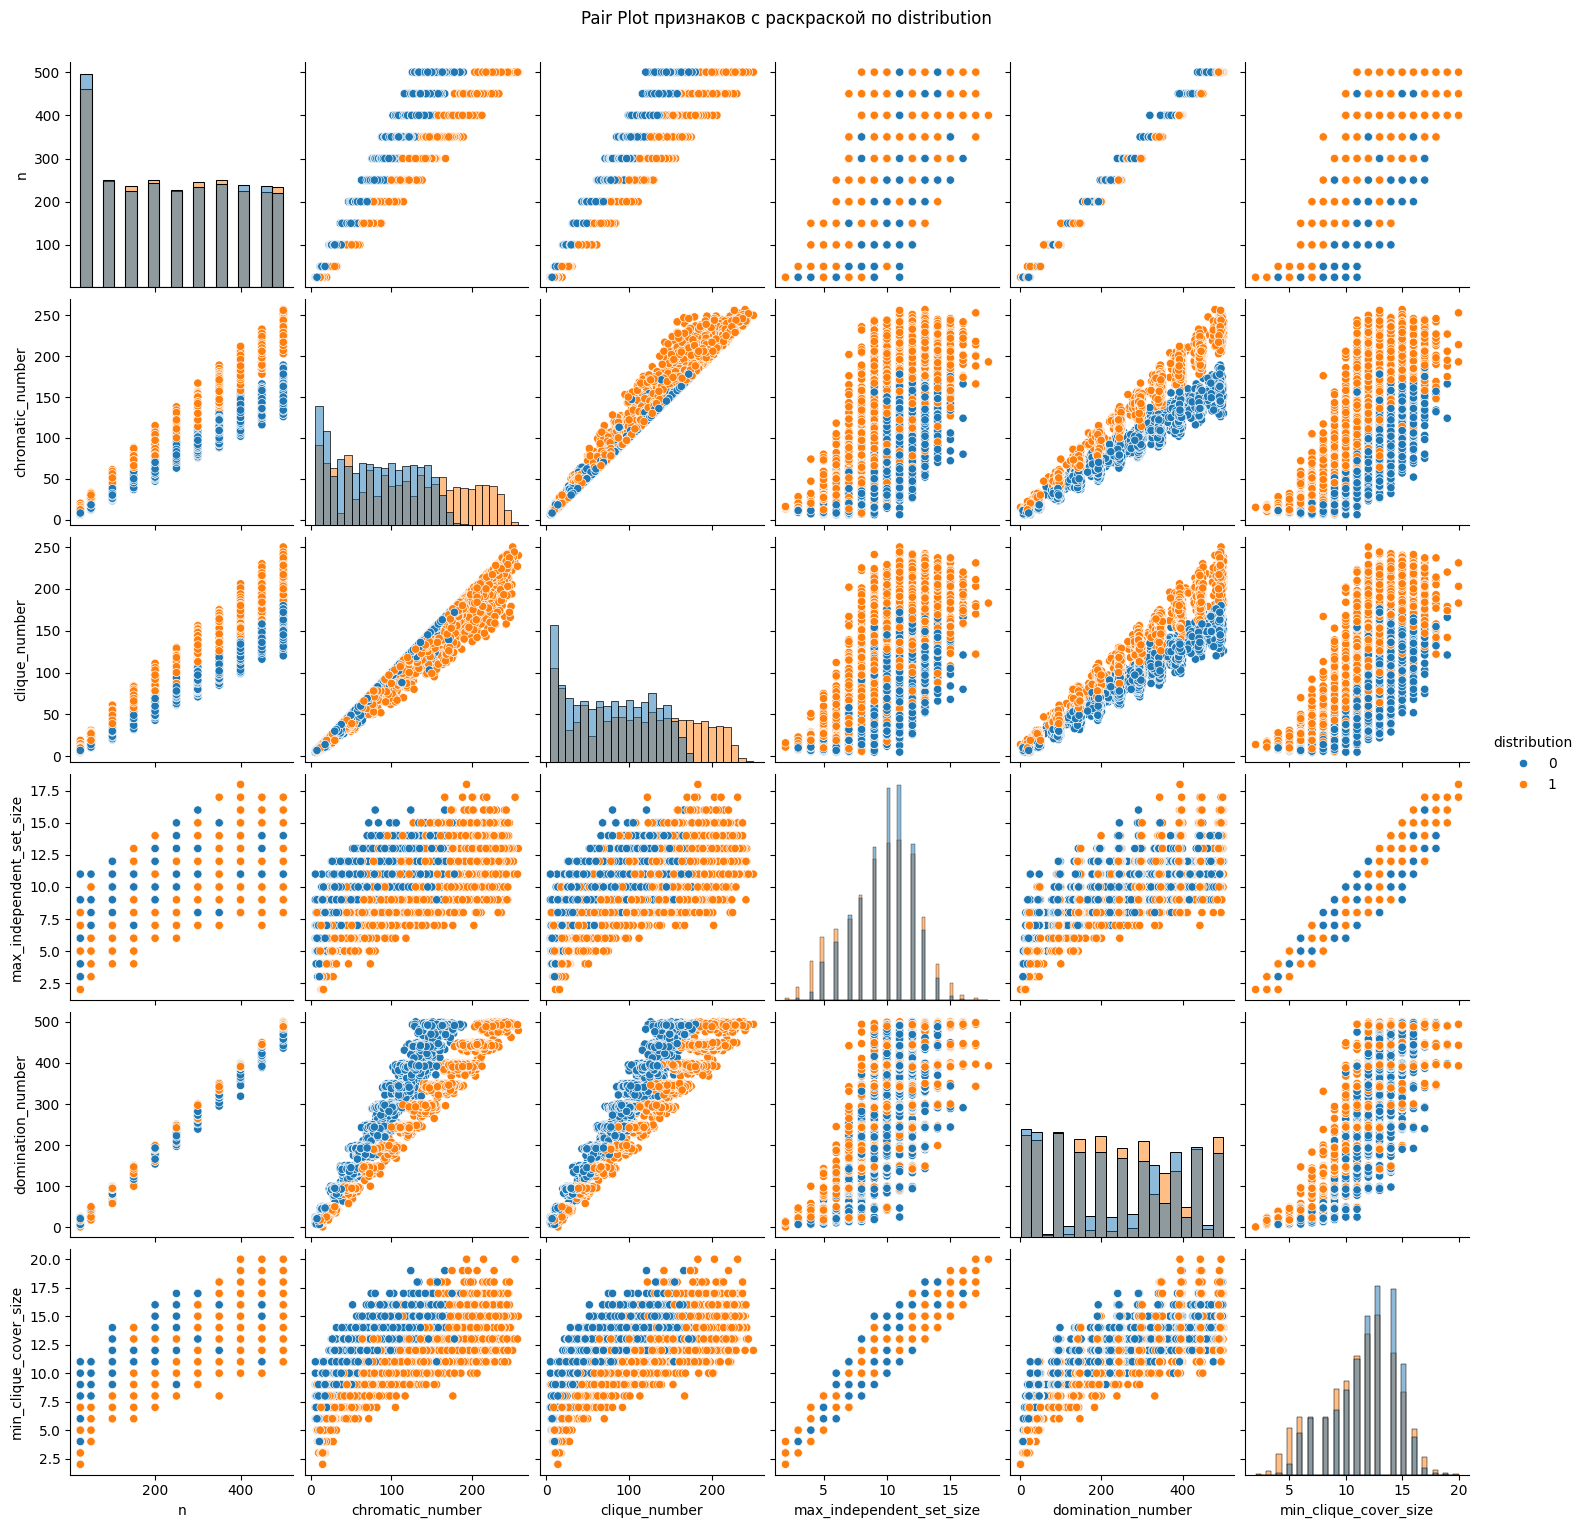
\includegraphics[width=1\linewidth]{img/dist-exp-lnorm.png}
Выводы:
\begin{itemize}
    \item Самые важные признаки для классификации: \texttt{chromatic\_number} и \texttt{clique\_number} (в нашем случае это одно и то же), они достаточно хорошо разделяют данную выборку на два класса при всех $n$;
    \item При росте $n$ важность характеристик не меняется, по-прежнему самый важный - \texttt{chromatic\_number}.
\end{itemize}
Между признаками прослеживаются зависимости:
\begin{itemize}
    \item \texttt{domination\_number} линейно зависит от \texttt{chromatic\_number};
    \item \texttt{max\_independent\_set\_size} и \texttt{min\_clique\_cover\_size} (в нашем случае это одно и то же) квадратично зависят от \texttt{domination\_number};
    \item \texttt{max\_independent\_set\_size} квадратично зависит от \texttt{chromatic\_number}.
\end{itemize}
Посмотрим на корреляции признаков:\\
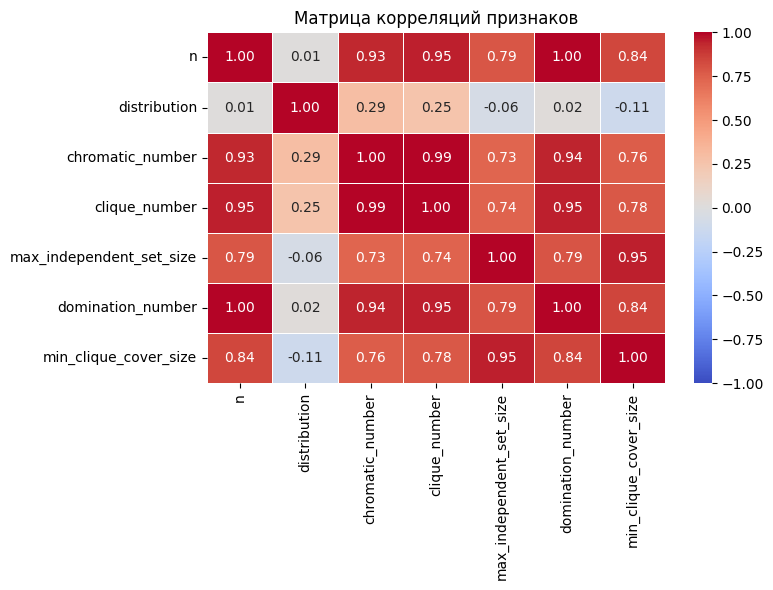
\includegraphics[width=1\linewidth]{img/corr-exp-lnorm.png}
Выводы:
\begin{itemize}
    \item В целом, тут мы можем найти подтверждения нашим выводам по pair plot;
    \item Больше всего с таргетом \texttt{distribution} коррелируют \texttt{chromatic\_number} и \texttt{clique\_number};
    \item \texttt{domination\_number} имеет сильную корреляцию со всеми остальными признаками и очень слабую с таргетом;
    \item \texttt{max\_independent\_set\_size} и \texttt{min\_clique\_cover\_size} имеют слабую корреляцию с таргетом, но довольно сильно зависят от других характеристик.
\end{itemize}
\subsection{\texttt{Normal(0, $\sigma$), SkewNormal($\alpha$)}}
Посмотрим на распределение таргета относительно признаков:\\
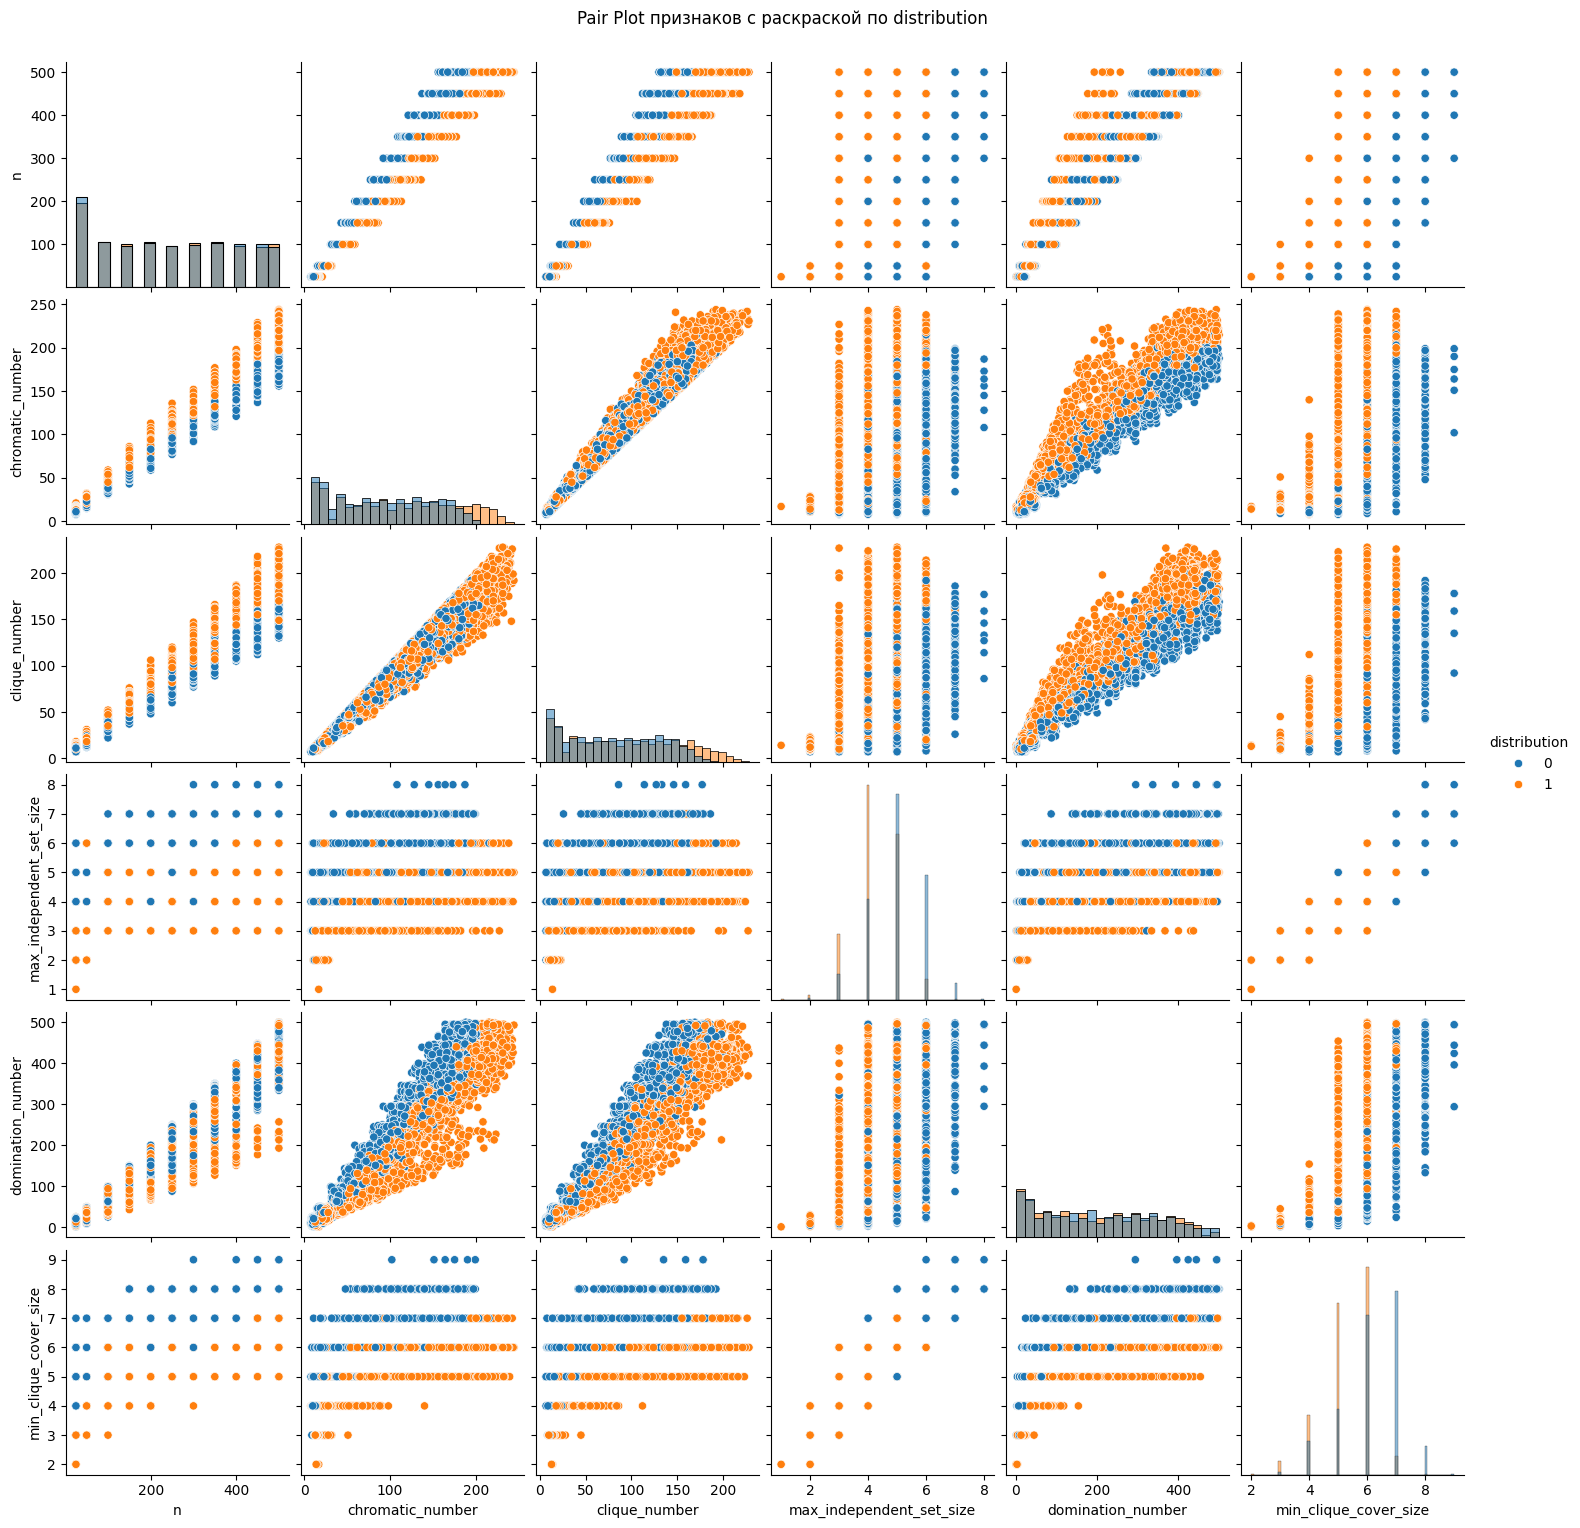
\includegraphics[width=1\linewidth]{img/dist-norm-snorm.png}
Аналогичные наблюдения.\\
Посмотрим на корреляции признаков:\\
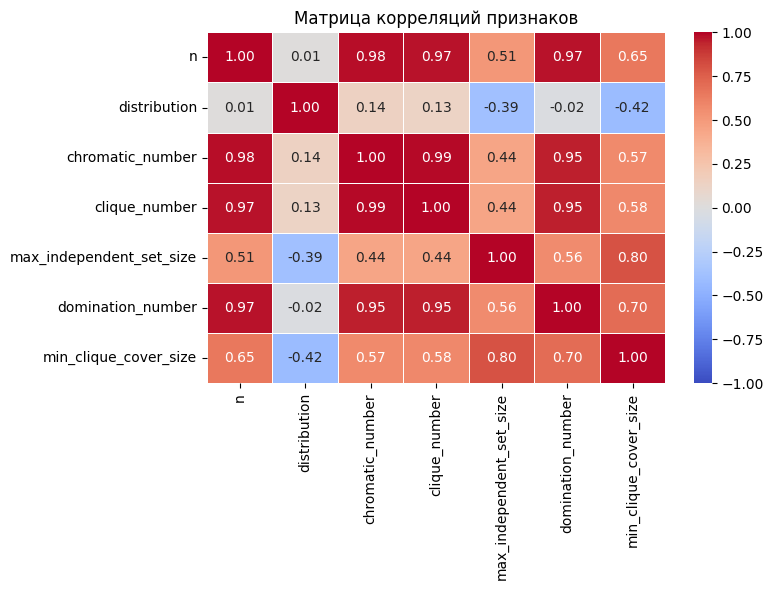
\includegraphics[width=1\linewidth]{img/corr-norm-snorm.png}
Выводы:
\begin{itemize}
    \item Получилось, что самая сильная корреляция с таргетом у \texttt{max\_independent\_set\_size} и \texttt{min\_clique\_cover\_size};
    \item \texttt{domination\_number} имеет сильную корреляцию со всеми остальными признаками и очень слабую с таргетом.
\end{itemize}
\subsection{Общие наблюдения}
Были предприняты попытки сгенерировать больше признаков путём нормирования, деления, возведения в квадрат и других операций, которые показались логичными в контексте конкретных признаков и их зависимости. В итоге особого прироста эффективности данная эвристика не дала, поэтому было принято решение обучать модели на изначальном датасете, взяв $n$ в качестве гиперпараметра модели.

\subsection{Выводы}
\begin{itemize}
    \item С поставленной задачей лучше всего справляется листанционный граф с параметром $d = 0.8$ для \texttt{Exp($\lambda$), LogNormal(0, $\sigma$)} и $d = 0.9$ для \texttt{Normal(0, $\sigma$), SkewNormal($\alpha$)};
    \item Значимость признаков не зависит от $n$, но при больших $n$ разделение становится более явным.
\end{itemize}

\section{Применение нескольких классификационных алгоритмов для фиксированного n}

В данном исследовании строился дистанционный граф с параметром $d = 0.8$ для \texttt{Exp($\lambda$), LogNormal(0, $\sigma$)} и $d = 0.9$ для \texttt{Normal(0, $\sigma$), SkewNormal($\alpha$)}, затем считались его характеристики и для фиксированного $n$ применялись три модели:
\begin{itemize}
    \item \texttt{LogisticRegression}
    \item \texttt{SVM}
    \item \texttt{RandomForestClassifier}
\end{itemize}

\subsection{$\text{n} = 25$}
\subsubsection{\texttt{Exp($\lambda$), LogNormal(0, $\sigma$)}}
\begin{table}[htbp]
  \centering
  \caption{Метрики разных моделей}
  \label{tab:results_exp_lognormal_25}
  \begin{tabular}{@{} l c c @{}}
    \toprule
    модель & мощность & ошибка первого рода \\
    \midrule
    LogisticRegression & 0.86 & 0.15 \\
    SVM                & 0.86 & 0.14 \\
    RandomForest       & 0.79 & 0.16 \\
    \bottomrule
  \end{tabular}
\end{table}

В таблице \ref{tab:results_exp_lognormal_25} приведены метрики для \texttt{Exp($\lambda$), LogNormal(0, $\sigma$)}, выводы:
\begin{itemize}
    \item Лучшие метрики показала SVM;
    \item Самый важный признак - хроматическое число.
\end{itemize}

\subsubsection{\texttt{Normal(0, $\sigma$), SkewNormal($\alpha$)}}
\begin{table}[htbp]
  \centering
  \caption{Метрики разных моделей}
  \label{tab:results_normal_skewnormal_25}
  \begin{tabular}{@{} l c c @{}}
    \toprule
    модель & мощность & ошибка первого рода \\
    \midrule
    LogisticRegression & 0.59 & 0.23 \\
    SVM                & 0.64 & 0.28 \\
    RandomForest       & 0.68 & 0.32 \\
    \bottomrule
  \end{tabular}
\end{table}

В таблице \ref{tab:results_normal_skewnormal_25} приведены метрики для \texttt{Normal(0, $\sigma$), SkewNormal($\alpha$)}, выводы:
\begin{itemize}
    \item Лучшие метрики показала логистическая регрессия;
    \item Самый важный признак - хроматическое число.
\end{itemize}

\subsection{$\text{n} = 100$}
\subsubsection{\texttt{Exp($\lambda$), LogNormal(0, $\sigma$)}}
\begin{table}[htbp]
  \centering
  \caption{Метрики разных моделей}
  \label{tab:results_exp_lognormal_100}
  \begin{tabular}{@{} l c c @{}}
    \toprule
    модель & мощность & ошибка первого рода \\
    \midrule
    LogisticRegression & 0.92 & 0.05 \\
    SVM                & 0.94 & 0.06 \\
    RandomForest       & 0.92 & 0.07 \\
    \bottomrule
  \end{tabular}
\end{table}

В таблице \ref{tab:results_exp_lognormal_100} приведены метрики для \texttt{Exp($\lambda$), LogNormal(0, $\sigma$)}, выводы:
\begin{itemize}
    \item Лучшие метрики показала SVM;
    \item Самый важный признак - хроматическое число.
\end{itemize}

\subsubsection{\texttt{Normal(0, $\sigma$), SkewNormal($\alpha$)}}
\begin{table}[htbp]
  \centering
  \caption{Метрики разных моделей}
  \label{tab:results_normal_skewnormal_100}
  \begin{tabular}{@{} l c c @{}}
    \toprule
    модель & мощность & ошибка первого рода \\
    \midrule
    LogisticRegression & 0.80 & 0.19 \\
    SVM                & 0.81 & 0.22 \\
    RandomForest       & 0.79 & 0.19 \\
    \bottomrule
  \end{tabular}
\end{table}

В таблице \ref{tab:results_normal_skewnormal_100} приведены метрики для \texttt{Normal(0, $\sigma$), SkewNormal($\alpha$)}, выводы:
\begin{itemize}
    \item Лучшие метрики показала логистическая регрессия с новыми признаками;
    \item Самый важный признак - минимальное кликовое покрытие разделить на хроматическое число.
\end{itemize}

\subsection{$\text{n} = 500$}
\subsubsection{\texttt{Exp($\lambda$), LogNormal(0, $\sigma$)}}
\begin{table}[htbp]
  \centering
  \caption{Метрики разных моделей}
  \label{tab:results_exp_lognormal_500}
  \begin{tabular}{@{} l c c @{}}
    \toprule
    модель & мощность & ошибка первого рода \\
    \midrule
    LogisticRegression & 1.0 & 0 \\
    SVM                & 1.0 & 0 \\
    RandomForest       & 1.0 & 0 \\
    \bottomrule
  \end{tabular}
\end{table}

В таблице \ref{tab:results_exp_lognormal_500} приведены метрики для \texttt{Exp($\lambda$), LogNormal(0, $\sigma$)}, выводы:
\begin{itemize}
    \item При достаточно больших $n = 500$ все алгоритмы могут определить гипотезу с очень хорошей вероятностью;
    \item Самый важный признак - хроматическое число.
\end{itemize}

\subsubsection{\texttt{Normal(0, $\sigma$), SkewNormal($\alpha$)}}
\begin{table}[htbp]
  \centering
  \caption{Метрики разных моделей}
  \label{tab:results_normal_skewnormal_500}
  \begin{tabular}{@{} l c c @{}}
    \toprule
    модель & мощность & ошибка первого рода \\
    \midrule
    LogisticRegression & 0.98 & 0.02 \\
    SVM                & 0.98 & 0.02 \\
    RandomForest       & 0.96 & 0.03 \\
    \bottomrule
  \end{tabular}
\end{table}

В таблице \ref{tab:results_normal_skewnormal_500} приведены метрики для \texttt{Normal(0, $\sigma$), SkewNormal($\alpha$)}, выводы:
\begin{itemize}
    \item Лучшие метрики показала логистическая регрессия с новыми признаками;
    \item Самый важный признак - минимальное кликовое покрытие разделить на хроматическое число.
\end{itemize}

% === Глава 4: Результаты ===
\chapter{Результаты}
Сделаем небольшие сводные таблицы с наилучшими результатами.
\begin{table}[htbp]
  \centering
  \caption{Результаты измерений для \texttt{Exp($\lambda$), LogNormal(0, $\sigma$)}}
  \label{tab:results_exp_lognormal}
  \begin{tabular}{@{} l c c @{}}
    \toprule
    n & мощность & ошибка первого рода \\
    \midrule
    25 & 0.86 & 0.14 \\
    100 & 0.94 & 0.06 \\
    500 & 1.0 & 0 \\
    \bottomrule
  \end{tabular}
\end{table}

\begin{table}[htbp]
  \centering
  \caption{Результаты измерений для \texttt{Normal(0, $\sigma$), SkewNormal($\alpha$)}}
  \label{tab:results_normal_skewnormal}
  \begin{tabular}{@{} l c c @{}}
    \toprule
    n & мощность & ошибка первого рода \\
    \midrule
    25 & 0.59 & 0.23 \\
    100 & 0.80 & 0.19 \\
    500 & 0.98 & 0.02 \\
    \bottomrule
  \end{tabular}
\end{table}

% === Глава 5: Заключение ===
\chapter{Заключение}
В ходе работы было установлено, что числовые характеристики случайных графов достаточно сильно влияют на распределение первоначальной выборки.\\\\
\textbf{Основные выводы:}
\begin{itemize}
  \item Рост $n$ значительно влият на качество классификатора, при больших $n$ мы можем делать более точные предсказания;
  \item Для некоторых распределений помогает преобразование старых и генерация новых признаков;
  \item Основные характеристики - хроматическая число и ее производные.
\end{itemize}

\end{document}
